% !TEX root = ../../../main.tex
% 来源：中学数学实验教材·第三册（高中数学）
% 章节：二次函数 / 和二次函数有关的课题
% 原始文件：5.tex，行 1516-1529
% 类型：tikz
% ---
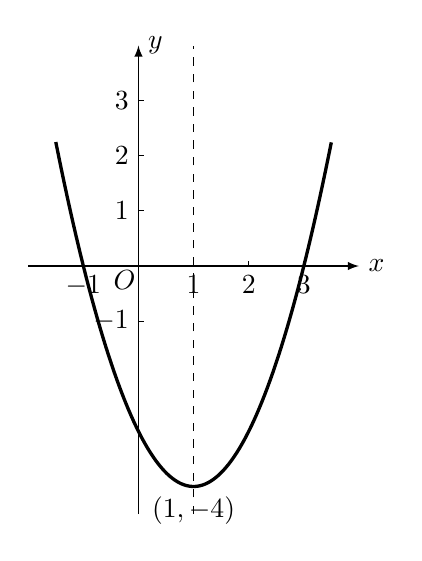
\begin{tikzpicture}[>=latex, scale=.7]
\draw[->] (-2,0)--(4,0)node[right]{$x$};
\draw[->] (0,-4.5)--(0,4)node[right]{$y$};
\foreach \x in {1,2,3,-1}
{
    \draw(\x,0)node[below]{$\x$}--(\x,.1);
    \draw(0,\x)node[left]{$\x$}--(.1,\x);
}       

\draw[dashed] (1,-4.5)--(1,4);
\draw [domain=-1.5:3.5, samples=100, very thick] plot(\x, {(\x-1)*(\x-1)-4});
\node at (1,-4)[below]{$(1,-4)$};
\node at (-.25,-.25){$O$};
    \end{tikzpicture}
